% Procedure for deinstallation

\stepcounter{tableCounter} % Increment counter
\setcounter{rowCounter}{0} % Reset counter
\begin{tabularx}{\textwidth}{|>{\columncolor{tableColumnColor}}c|>{\columncolor{tableColumnColor}}c|>{\columncolor{tableColumnColor}}c|>{\columncolor{tableColumnColor}}c|X|}
  \hline
  \rowcolor{tableHeaderColor}
  ID & CK 1 & CK 2 & CK 3 & Description \\ \hline

  \procedureItem{
    After ROS has been stopped, navigate to the \texttt{catkin\_ws/src/rosbags} folder and to the following:
    \begin{itemize}
      \item select all files (CTRL-A), right-click and select Compress...

      \item select .zip and name the file according to the test designation. Save it in the same rosbags folder.
            \\
            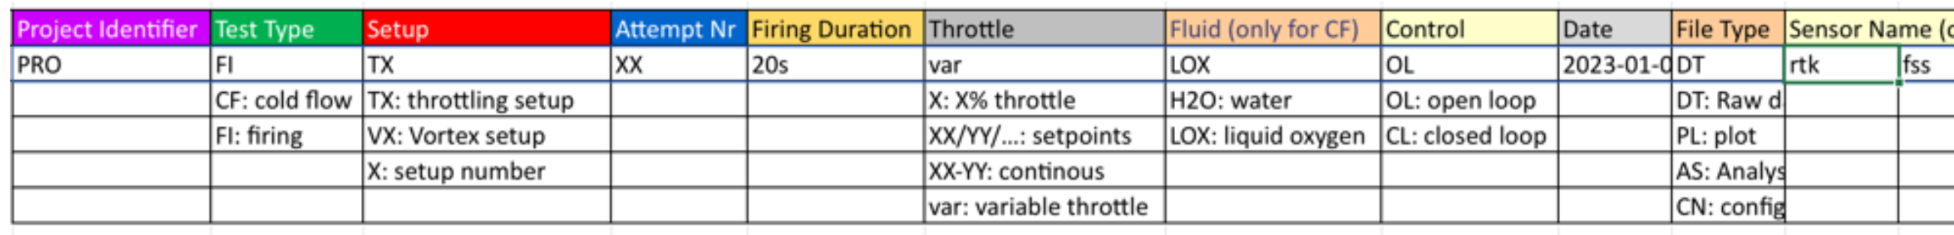
\includegraphics[width=0.5\textwidth]{assets/table-screenshot.png}


      \item if it complains about a file with an .active extension, just delete that file and try again

      \item Upload this .zip file to sharepoint into the folder /Data/\textless testtype\textgreater /\textless specifictest\textgreater  (see installation)

      \item As well as move this file to the folder catkin\_ws/src/archivedbags

      \item Double check that you uploaded this data correctly

      \item select all files in the rosbags folder and delete them
    \end{itemize}
  }

  \procedureItem{
    Save the Config file in \texttt{/home/git/configuration\_tests} to the folder mentioned above (Data/ testfolder/Configuration)
  }

  \procedureItem{
    Save test \texttt{list.csv} and \texttt{test\_sequences.csv} in
    \texttt{/home/git/software-rpi4/state\_machine/src}
    to the folder mentioned above (Data/ testfolder/Configuration)
  }

  \procedureItem{
    Save the videos from the screen recordings and potential screenshots in the Videos or Pictures folder
  }

  \procedureItem{
    Save the ROS graphs created during the test in the corresponding folder in sharepoint inside a new folder named ROS Plots
  }

  \procedureItem{
    Download recorded video material from surveillance modem (can also be done at a later point)
  }
\end{tabularx}
